\documentclass[tikz, border=20pt]{standalone}
\usepackage{amsmath, amssymb}
\usetikzlibrary{shapes.geometric, arrows.meta, positioning, fit, calc, backgrounds, shadows.blur}

\begin{document}
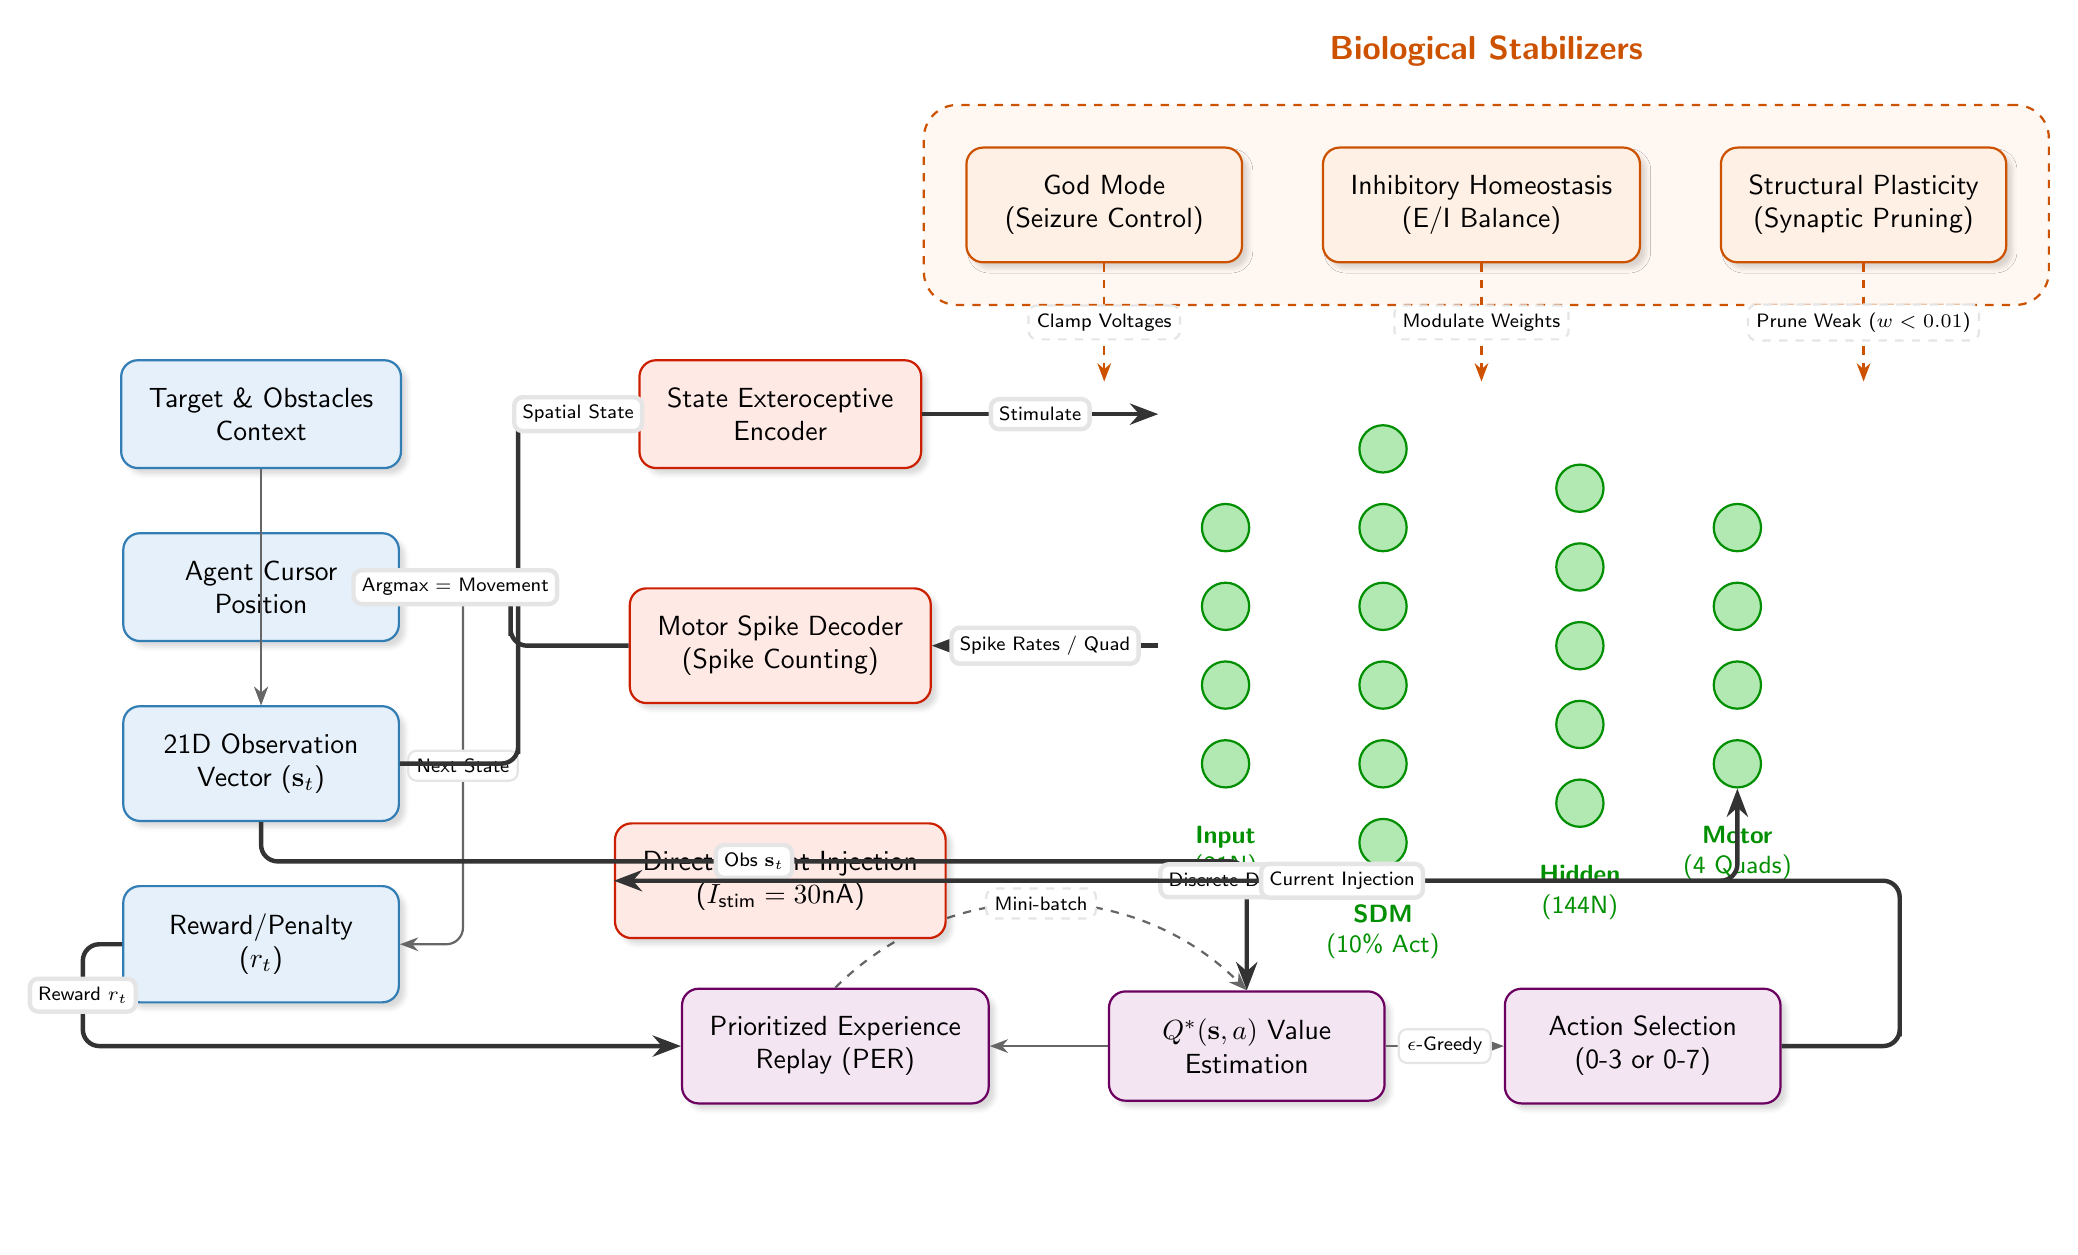
\begin{tikzpicture}[>=Stealth,
    node distance=1.5cm and 2cm,
    font=\sffamily,
    % Box styles
    box/.style={
        rectangle, rounded corners=6pt, thick,
        draw=#1!80!black, fill=#1!10, text=black,
        align=center, inner sep=10pt, minimum width=3.5cm, minimum height=1.2cm,
        blur shadow={shadow opacity=15, shadow blur steps=3}
    },
    % Group styles
    group/.style={
        rectangle, rounded corners=12pt, thick, dashed,
        draw=#1!80!black, fill=#1!5, inner sep=15pt
    },
    title/.style={font=\sffamily\bfseries\large, text=#1!80!black},
    % Edge styles
    edge norm/.style={->, thick, draw=black!60, rounded corners=6pt},
    edge bold/.style={->, ultra thick, draw=black!80, rounded corners=6pt},
    edge dash/.style={->, thick, dashed, draw=black!60, rounded corners=6pt},
    lbl/.style={fill=white, font=\sffamily\scriptsize, inner sep=3pt, rounded corners=3pt, draw=black!10, align=center},
    % Neural network styles
    neuron/.style={circle, draw=#1!80!black, fill=#1!30, thick, minimum size=0.6cm, inner sep=0pt}
]

% Define base colors
\colorlet{env}{cyan!70!blue}
\colorlet{agt}{purple!70!blue}
\colorlet{int}{red!70!orange}
\colorlet{snn}{green!70!black}
\colorlet{stb}{orange!80!red}

% ====================
% 1. ENVIRONMENT (Left)
% ====================
\node[box=env] (e_tar) {Target \& Obstacles\\Context};
\node[box=env, below=0.8cm of e_tar] (e_cur) {Agent Cursor\\Position};
\node[box=env, below=0.8cm of e_cur] (e_obs) {21D Observation\\Vector ($\mathbf{s}_t$)};
\node[box=env, below=0.8cm of e_obs] (e_rew) {Reward/Penalty\\($r_t$)};

\begin{scope}[on background layer]
    \node[group=env, fit=(e_tar) (e_rew) (e_obs)] (e_grp) {};
    \node[title=env, above=10pt of e_grp.north] {Environment};
\end{scope}

\draw[edge norm] (e_tar) -- (e_obs);
\draw[edge norm] (e_cur) -- (e_obs);
\draw[edge norm] (e_cur.east) -- ++(0.8,0) |- node[lbl, pos=0.25] {Next State} (e_rew.east);


% ====================
% 2. OUTER AGENT (Bottom)
% ====================
\node[box=agt, right=3cm of e_grp.south east, anchor=west] (a_per) {Prioritized Experience\\Replay (PER)};
\node[box=agt, right=1.5cm of a_per] (a_q) {$Q^*(\mathbf{s}, a)$ Value\\Estimation};
\node[box=agt, right=1.5cm of a_q] (a_act) {Action Selection\\(0-3 or 0-7)};

\begin{scope}[on background layer]
    \node[group=agt, fit=(a_per) (a_act)] (a_grp) {};
    \node[title=agt, below=10pt of a_grp.south] {Outer Control Agent (Dueling DDQN)};
\end{scope}

\draw[edge norm] (a_q) -- node[lbl] {$\epsilon$-Greedy} (a_act);
\draw[edge norm] (a_q) -- (a_per);
\draw[edge dash] (a_per.north) to[out=45, in=135] node[lbl] {Mini-batch} (a_q.north);


% ====================
% 3. INTERFACE (Middle Top)
% ====================
\node[box=int, right=3cm of e_tar.east, anchor=west] (i_enc) {State Exteroceptive\\Encoder};
\node[box=int, below=1.5cm of i_enc] (i_dec) {Motor Spike Decoder\\(Spike Counting)};
\node[box=int, below=1.5cm of i_dec] (i_inj) {Direct Current Injection\\($I_{\text{stim}} = 30\text{nA}$)};

\begin{scope}[on background layer]
    \node[group=int, fit=(i_enc) (i_inj)] (i_grp) {};
    \node[title=int, above=10pt of i_grp.north] {Sensory-Motor Interface};
\end{scope}


% ====================
% 4. ORGANOID SNN (Right)
% ====================
% Coordinates for neural network based on the Interface block
\coordinate (snn_center) at ([xshift=6cm]i_grp.east |- i_dec);

\def\xIn{-3}
\def\xSdm{-1}
\def\xHid{1.5}
\def\xMot{3.5}

\begin{scope}[shift={(snn_center)}]
    % Input Layer (4 nodes)
    \foreach \i/\y in {1/1.5, 2/0.5, 3/-0.5, 4/-1.5} {
        \node[neuron=snn] (n_in_\i) at (\xIn, \y) {};
    }
    \node[text=snn!80!black, font=\sffamily\small, align=center, below=10pt of n_in_4] {\textbf{Input}\\(21N)};

    % SDM Layer (6 nodes)
    \foreach \i/\y in {1/2.5, 2/1.5, 3/0.5, 4/-0.5, 5/-1.5, 6/-2.5} {
        \node[neuron=snn] (n_sd_\i) at (\xSdm, \y) {};
    }
    \node[text=snn!80!black, font=\sffamily\small, align=center, below=10pt of n_sd_6] {\textbf{SDM}\\(10\% Act)};

    % Hidden Layer (5 nodes)
    \foreach \i/\y in {1/2.0, 2/1.0, 3/0, 4/-1.0, 5/-2.0} {
        \node[neuron=snn] (n_hd_\i) at (\xHid, \y) {};
    }
    \node[text=snn!80!black, font=\sffamily\small, align=center, below=10pt of n_hd_5] {\textbf{Hidden}\\(144N)};

    % Motor Layer (4 nodes)
    \foreach \i/\y in {1/1.5, 2/0.5, 3/-0.5, 4/-1.5} {
        \node[neuron=snn] (n_mt_\i) at (\xMot, \y) {};
    }
    \node[text=snn!80!black, font=\sffamily\small, align=center, below=10pt of n_mt_4] {\textbf{Motor}\\(4 Quads)};

    % Connectivity
    \begin{scope}[on background layer]
        % In -> SDM
        \foreach \i in {1,...,4} {
            \foreach \j in {1,...,6} {
                % sparse-ish appearance by not drawing all
                \pgfmathparse{mod(\i+\j,3)==0 ? 1 : 0}
                \ifnum\pgfmathresult=1
                    \draw[->, snn!30] (n_in_\i) -- (n_sd_\j);
                \fi
            }
            \draw[->, snn!30] (n_in_\i) -- (n_sd_\i);
        }
    
        % SDM -> Hidden
        \foreach \i in {1,...,6} {
            \foreach \j in {1,...,5} {
                \draw[->, snn!20] (n_sd_\i) -- (n_hd_\j);
            }
        }
    
        % Hidden -> Hidden
        \foreach \i in {1,...,5} {
            \draw[->, snn!80] (n_hd_\i) to[out=45, in=315, looseness=4] (n_hd_\i);
        }
        
        % Hidden -> Motor
        \foreach \i in {1,...,5} {
            \foreach \j in {1,...,4} {
                \draw[->, snn!40] (n_hd_\i) -- (n_mt_\j);
            }
        }
    \end{scope}
\end{scope}

\begin{scope}[on background layer]
    \node[group=snn, fit=(n_sd_1) (n_sd_6) (n_mt_1) (n_mt_4) (n_in_1)] (s_grp) {};
    \node[title=snn, above=10pt of s_grp.north] {The Organoid (Metabolic-Izhikevich SNN)};
\end{scope}


% ====================
% 5. BIOLOGICAL STABILIZERS (Top)
% ====================
\node[box=stb, above=1.5cm of s_grp] (t_hom) {Inhibitory Homeostasis\\(E/I Balance)};
\node[box=stb, left=1cm of t_hom] (t_god) {God Mode\\(Seizure Control)};
\node[box=stb, right=1cm of t_hom] (t_pla) {Structural Plasticity\\(Synaptic Pruning)};

\begin{scope}[on background layer]
    \node[group=stb, fit=(t_god) (t_hom) (t_pla)] (t_grp) {};
    \node[title=stb, above=10pt of t_grp.north] {Biological Stabilizers};
\end{scope}


% ====================
% 6. CROSS-SYSTEM CONNECTIONS
% ====================

% Env -> Agent
% e_obs is on the left, a_q is on the bottom. We route from e_obs south to a_q.
\draw[edge bold] (e_obs.south) -- ++(0,-0.5) -| node[lbl, pos=0.25] {Obs \(\mathbf{s}_t\)} (a_q.north);
\draw[edge bold] (e_rew.west) -- ++(-0.5,0) |- node[lbl, pos=0.25] {Reward \(r_t\)} (a_per.west);

% Env -> Interface
\draw[edge bold] (e_obs.east) -| ++(1.5, 0) |- node[lbl, pos=0.75] {Spatial State} (i_enc.west);

% Agent -> Interface
\draw[edge bold] (a_act.east) -| ++(1.5, 0) |- node[lbl, pos=0.75] {Discrete Decision \(a_t\)} (i_inj.west);

% Interface -> SNN
\coordinate (snn_in_port) at (s_grp.west |- i_enc.east);
\draw[edge bold] (i_enc.east) -- node[lbl] {Stimulate} (snn_in_port);

% Current injection -> SNN motor layer
\draw[edge bold] (i_inj.east) -| node[lbl, pos=0.25] {Current Injection} (n_mt_4.south);

% SNN -> Interface
\coordinate (snn_out_port) at (s_grp.west |- i_dec.east);
\draw[edge bold] (snn_out_port) -- node[lbl] {Spike Rates / Quad} (i_dec.east);

% Interface -> Env
\draw[edge bold] (i_dec.west) -| ++(-1.5, 0) |- node[lbl, pos=0.75] {Argmax = Movement} (e_cur.east);

% Stabilizers -> SNN
\draw[edge dash, draw=stb!80!black] (t_god.south) -- node[lbl] {Clamp Voltages} (t_god.south |- s_grp.north);
\draw[edge dash, draw=stb!80!black] (t_hom.south) -- node[lbl] {Modulate Weights} (t_hom.south |- s_grp.north);
\draw[edge dash, draw=stb!80!black] (t_pla.south) -- node[lbl] {Prune Weak ($w<0.01$)} (t_pla.south |- s_grp.north);

\end{tikzpicture}
\end{document}
